\documentclass[12pt]{article}
\input{\string~/.macros}
\usepackage{hyperref}
\hypersetup{
    colorlinks=true,
    linkcolor=blue,
    filecolor=blue,      
    urlcolor=blue,
}
\usepackage[a4paper, total={7in, 9in}]{geometry}

\usepackage{graphicx}   % incorporating graphics
\graphicspath{{assets/}}


\newcommand{\lgh}[1]{
    \href{https://github.com/tt6746690/sparse_solver/blob/master/#1}{\texttt{#1}}
}
\newcommand{\lghh}[2]{
    \href{https://github.com/tt6746690/sparse_solver/blob/master/#1}{\texttt{#2}}
}


\begin{document}

\begin{center}
    {\Large 
        Report for 2019 applicants by Peiqi Wang
    }
\end{center}
This report explains my efforts in trying to implement forward substitution method on sparse matrices. Sequantially, I made the following implementations \href{https://github.com/tt6746690/sparse_solver}{here}

\begin{enumerate}
    \item (\lgh{src/formats.h}) I/O code for interfacing with Matrix Market format files
    \item (\lgh{tests.cpp}) tests that verifies the correctness of the method
    \item (\lgh{src/triangular.h}) forward substitution method that relies on finding the reachset
    \item (\lgh{src/triangular.h}) a method that relies on \texttt{OpenMP} naively
    \item (\lgh{scripts/codegen.ipynb}) code generation routine that takes into account sparsity patterns
\end{enumerate}


\section{The Problem}

Find efficient methods to solve $\bL\bx = \bb$ where both $\bL, \bb$ are sparse and $\bL$ is lower triangular

\section{Verification Strategies}

I implemented two verification strategies (\lgh{tests.cpp\#L126})
\begin{enumerate}
    \item (\lgh{tests.cpp\#L136}) Given a tentative solution $\bx$, compute $\bL \bx$ and show $\bL\bx \approx \bb$
    \item (\lgh{scripts/triangular.m\#L23}) Compute $\bL \backslash \bb$ in MATLAB (and Julia) and show $\bx \approx \bL \backslash \bb$
\end{enumerate}
I noticed that strategy (1) show agreement for small matrices but indicates that $\bx$ is computed incorrectly for large matrices. After some debugging, I found that the matrix accumulates error and are ill-conditioned (verified with \lgh{scripts/cond.m}). During testing, (1) is tested against small matrices while (2) is tested against all available matrices (that I tried).

\section{Code Generation}

Two purpose of code generation in this specific problem
\begin{enumerate}
    \item reduce array access since position of nonzero values in $\bL,\bb$ are known beforehand
    \item allow for low level optimizations such as loop peeling, vectorization, etc.
\end{enumerate}
I code up a script to generate some code for \texttt{torso} and \texttt{tsopf}. However I only managed to achieve goal (1) and partially goal (2). The code never finishes compilation when \texttt{-O3} is set so goal (2) is only partially achieved by manual loop peeling during the code generation process.


\section{Methods and Results}

Several variations of forward substitution are compared
\begin{enumerate}
    \item (\lghh{src/triangular.h\#L45}{lsolve\_simple}) does not consider sparsity
    \item (\lghh{src/triangular.h\#L48}{lsolve\_eigen}) updates to nonzero values in $j$-th column of $\bL$ is skipped if $\bx_k$ is 0
    \item (\lghh{src/triangular.h\#L51}{lsolve\_reachset\_default})
    \begin{itemize}
        \item (\textit{symbolic}) computes $\texttt{Reach}_L(\bb) = \pc{j \mid \bx_j \neq 0}$ using depth-first-search
        \item (\textit{numeric}) performs numerical solve in topological order of $\texttt{Reach}_L(\bb)$
    \end{itemize}
    \item (\lghh{src/triangular.h\#L55}{lsolve\_reachset\_\{small,medium,torso,tsopf\}}) are variants of (3); code is generated with information of sparsity pattern of matrix. For now, the generated code has loop peeled manually, by referencin the Sympiler paper. Vectorization, tiling, etc. are not implemented as compiler directives as I am not too familiar with them
    \item (\lghh{src/triangular.h\#L69}{lsolve\_eigen\_par}) has inner loop naively wrapped in a \texttt{\#pragma omp parallel for}
\end{enumerate}
Performance of above methods are compared by running each method 10 times, whereby average is taken and normalized to that of \texttt{solve\_simple}. Two sparse matrix lhs are used as inputs, specifically \href{https://sparse.tamu.edu/Norris/torso1}{torso} and \href{https://sparse.tamu.edu/TSOPF/TSOPF_RS_b678_c2}{tsopf}. Code is compiled on MacOS 10.13.6 with Clang with \texttt{-O0}. As mentioned previously, it takes too long to compile code with \texttt{-O3} since file size for generated files is too large, i.e. \lgh{src/codegen\_torso.cpp} is approximately \texttt{3.5MB}. \\
From Figure~\ref{fig:1}, we see 
\begin{enumerate}
    \item significant performance gain for all other methods from using reachset for \texttt{tsopf}, and moderate performance for \texttt{lsolve\_eigen} and the reachset based methods. This is due to the fact that \texttt{torso} has a lot more nonzero elements; both numeric and symbolic time for sparse matrix increases with the number of nonzero elements. 
    \item \texttt{lsolve\_eigen} is simple to implement and performs quite well in these two cases. This is due to the fact that certain loops are skipped and runtime $O(n) \rightarrow O(nnz)$
    \item \texttt{lsolve\_reachset\_torso} has a slightly better numeric runtime performance when compared to \texttt{lsolve\_reachset\_default}, this is mostly due to the fact that code generation removes quite a number of array access operations. The code could get even faster if vectorization, tiling and other optimization methods are enabled.
    \item \texttt{lsolve\_eigen\_par} is my only attempt to parallelize the code and a bad one. The performance is worse due to extra cost of thread creation, synchronization, and communication. Additionally, threads do not have enough work to do before they are synchronized to enter the next outer loop. Something I would probably have tried is something that ParSy have come up with, i.e. coarse level parallelism to decrease synchronization cost while preserving data dependency
\end{enumerate}

  
\begin{figure}[ht]
    \begin{center}
        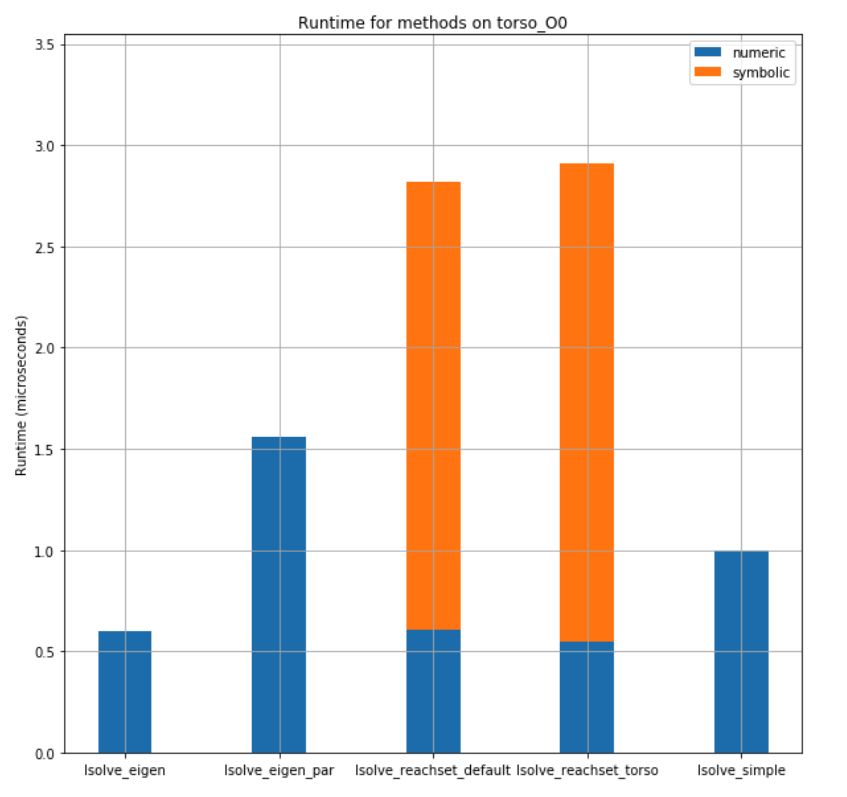
\includegraphics[width=5in]{runtime_torso_O0.png}
        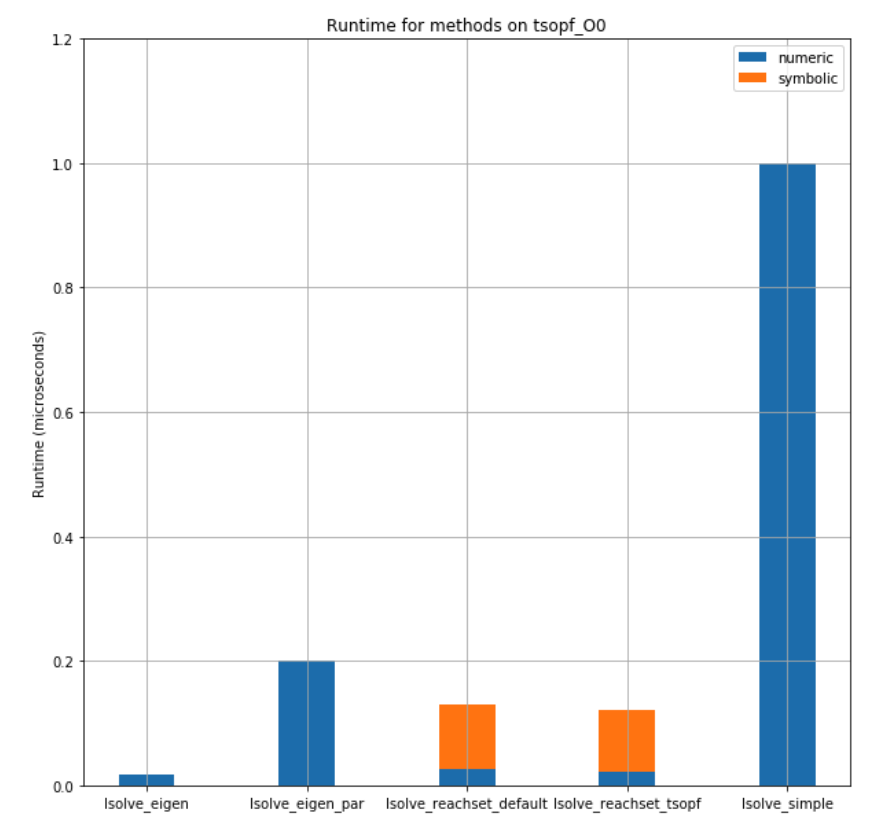
\includegraphics[width=5in]{runtime_tsopf_O0.png}
    \end{center}
    \caption{\label{fig:1} runtime on \texttt{torso} and \texttt{tsopf} with \texttt{-O0}}
\end{figure}



\end{document}
